\chapter{Data analysis}
\section{Data selection}

In this chapter we outline the selection criteria applied for this analysis. Basically, we used LHC10 data with pass 2 reconstruction which marked as "good run". The period of data taking is LHC10h and it is only data sets from heavy-ion collisions from 2010. 

Also we are using simulation data sets for MC studies, which are named  AMPT13f3a, AMPT13f3b, AMPT13f3c, and HIJING which correspond to the LHC10h data


\subsection{Default cuts and settings}

See bellow for default track selection,  event selection and cut criteria settings used in this analysis and the reason for these settings

\begin{itemize}
\item MC study
	\begin{itemize}
		\item {$-10 cm <Z_{vtx}<10 cm$}
		\item Track selection bit : IsPhysicalPrimary()
		\item $|\eta| < 0.8$
		\item Use Impact parameter information (see below tables )
		\item All charged particles except weak decaying particles
		\item $0.2 < p_{T} < 5.0$ GeV/$c$
		\item Collision Candidates : AliVEvent::kAny
	\end{itemize}
	
\item Data Analysis
	\begin{itemize}
		\item  $-10 cm <Z_{vtx}<10 cm$
		\item Track selection bit : TPC Only Filterbit(128)
		\item $\eta < 0.8$
		\item V0M centrality estimator
		\item All charged particles
		\item $0.2 < p_{T} < 5.0$ GeV/$c$
		\item Collision Candidates : AliVEvent::kMB
	\end{itemize}
\end{itemize}


\begin{center} \tiny{
\begin{tabular}{ |c|c c c c c c c c| } 
 \hline
Centrality(\%)&0-5      &5-10     &10-20    &20-30    &30-40     &40-50      &50-60      &60-70\\ 
\hline
b(fm) AMPT    &0.00-3.72&3.72-5.23&5.23-7.31&7.31-8.88&8.88-10.20&10.20-11.38&11.38-12.47&12.47-13.50\\ 
b(fm) HIJING  &0.00-3.60&3.60-5.09&5.09-7.20&7.20-8.83&8.83-10.20&10.20-11.40&11.40-12.49&12.49-13.49\\ 
b(fm) ALICE   &0.00-3.50&3.50-4.94&4.94-6.98&6.98-    &    -9.88 &9.81-      &     -12.09&12.09-\\
 \hline
\end{tabular}
\url{https://twiki.cern.ch/twiki/bin/viewauth/ALICE/CentStudies}
\label{table:impact} }
\end{center}

For the primary vertex determinations were performed by the ALICE ITS detector, in particular with its innermost part the SPD. The resolution in the z-coordinate is at the level of 10$\mu$m. In heavy-ion collision usually events with a primary vertex found in $|z| < 10$cm were used for most of ALICE analysis to ensure an uniform acceptance in the central pseudorapidity region.

The default estimator for centrality determination in ALICE is obtained from the measurement multiplicity in the VZERO detectors. Other centrality estimators such as those based on multiplicity measurement in the SPD or TPC detectors will be used for the systematic uncertainty estimate.

Also, even though the Inner tracking System (ITS) and the Time Projection Chanmber (TPC) were used as the main tracking devices for ALICE experiment, ITS does not have uniform acceptance. On the other hand, corrections for TPC are negligible due to its uniform acceptance. Because of this, we are going to use TPC only cuts, in which the tracks are required to have at least 70 reconstructed space point out of the maximum 159 in the TPC and a $\langle \chi^2 \rangle$ per TPC cluster $\le 4$ (with 2 degrees of freedom per cluster)


\vskip20mm
\subsection{Data QA}

\subsubsection{ $\eta$ distribution QA} 

 In principle, the multiplicity in each $\eta$ region should be similar(i.e. $N_{Aside} \sim N_{Cside}$). To confirm this similarity of multiplicity in each $\eta$ set, we check $\eta$ distribution for each centrality bins. Also the multiplicity in $\eta < 0$ region  and $\eta > 0$ is compared with filp over $\eta$ values as ratio. The below figures are the $\eta$ distribution for run number 137135. 


	\begin{figure}[!h]
		\begin{center}
        	\resizebox{0.86\columnwidth}{!}{\includegraphics{figures/figs_QA/eta_ratio_run137135_eta_04_08.eps}}
        	\caption{$dN/d\eta$ for flip over +/- $\eta$ region}
        	\label{dNdetaQA}
        \end{center}
    \end{figure}


     \begin{figure}[!h]
		\begin{center}
        	\resizebox{0.86\columnwidth}{!}{\includegraphics{figures/figs_QA/eta_ratio_run137135_eta_04_08.eps}}
        	\caption{fit result from ratio of $0.4<|\eta|<0.8$}
        	\label{dNdeta_ratio_fitQA}
        \end{center}
    \end{figure}


The ratio between number of multiplicity in $\eta>0 $ subgroup and $\eta<0$ subgroups,
was fitted with 0th order polynomial function with unity parameter(i.e $y=1$) run by run. After fitting, $\chi^2 / NDF$ was calculated to check for the same multiplicity in both subset groups for each run, each centralities. 

	
     \begin{figure}[hp]
		\begin{center}
        	\resizebox{0.85\columnwidth}{!}{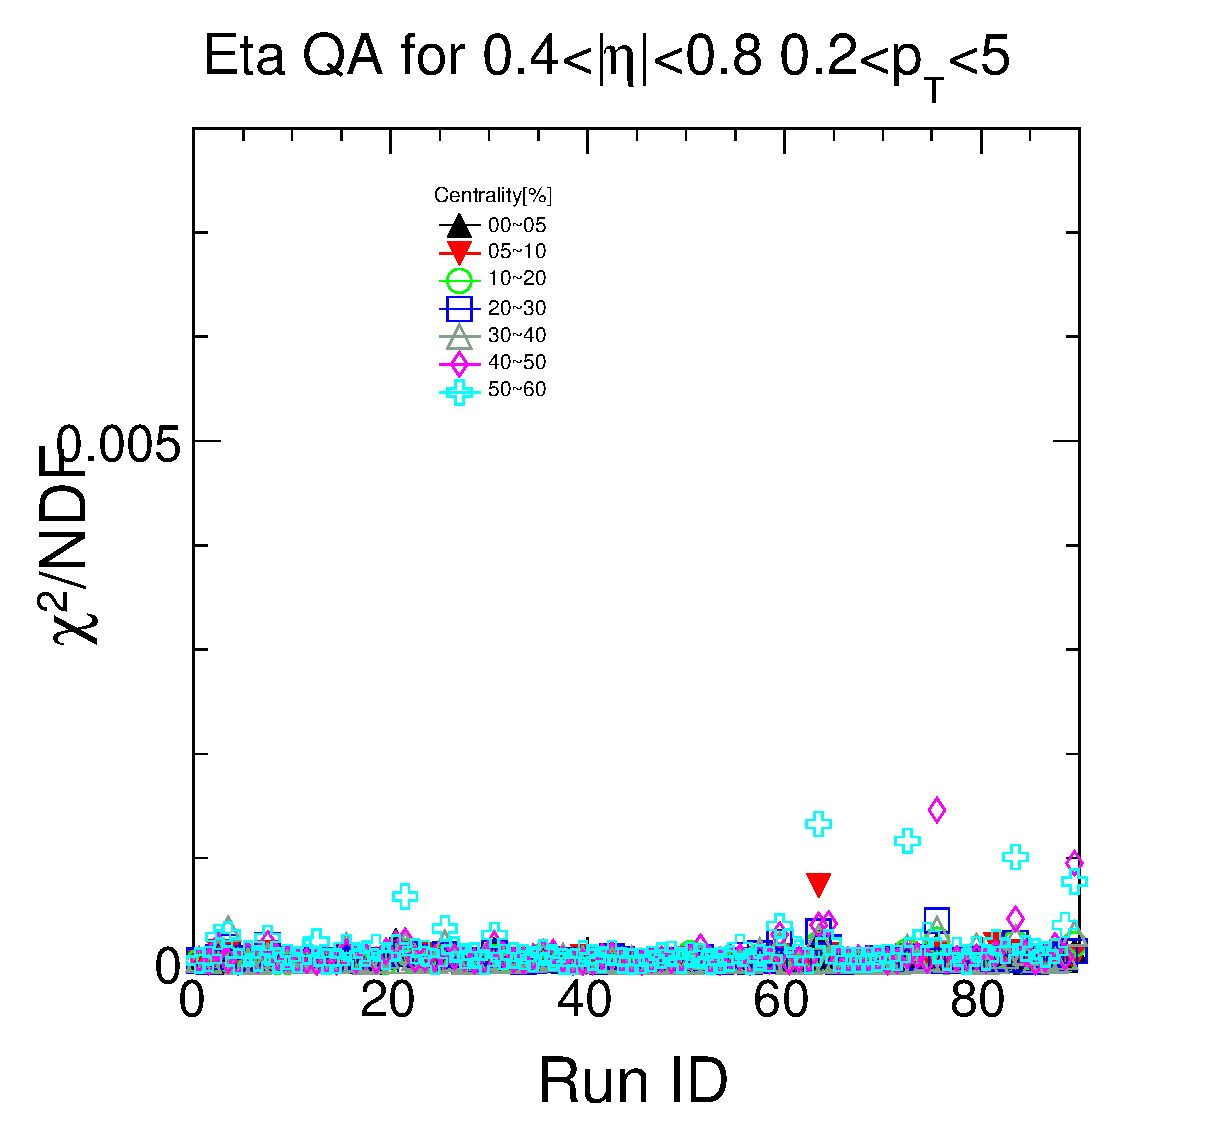
\includegraphics{figures/figs_QA/QA_Eta_ratio_flatness_LHC10h_AOD86.eps}}
        	\caption{$\chi^2/NDF$ for $\eta$ flatness}
        	\label{eta_flatnessQA}
        \end{center}
    \end{figure}

The results are shown in the figure as a function of RunID(instead of run number, corresponding run number can be found in Appendix)
QA result looks quite good across the runs as shown in figure. $\chi^2/NDF$ was lower than 0.002 for all runs and all centralities. We might simply assume that number of multiplicity in each subgroups are same.



\subsubsection{ $\phi$ distribution QA}

 $\phi$ flatness QA was performed on the $\phi$ distributions with LHC10h period data. We fit the distributions with 0th-order polynomial. The distribution was fitted run by run. $\chi^2/NDF$ was taken to estimate the flatness of distribution as like $\eta$ QA method. The fit results are shown in the below figure. 
 
    \begin{figure}[hp]
		\begin{center}
        	\resizebox{0.45\columnwidth}{!}{\includegraphics{figures/figs_QA/QA_RbR_phi_Aside_LHC10h_AOD86.eps}}
        	\resizebox{0.45\columnwidth}{!}{\includegraphics{figures/figs_QA/QA_RbR_phi_Cside_LHC10h_AOD86.eps}}
        \caption{$\chi^2/NDF$ for $\phi$ flatness for $\eta < 0$(left) and $\eta > 0$(right)}
        \label{fig:QC_phi_chi2NDF}
        \end{center}   
     \end{figure}

As shown in the figure, the flatness ($\chi^2/NDF$ of $\phi$) of some runs is worse then others. This is  considered as a detector effect, and might be affect on our analysis. The effect of non-uniform $\phi$ distribution will be treated as systematics.
 
 



\clearpage
\section{Analysis strategy}
\label{sec:analysis}

Recently, we reported new key observable for correlations between different order flow harmonics which is named ``Symmetric 2-harmonic 4-particle Cumulants(SC)".  This new observable are based on 4-particle cumulant, and defined as 

\begin{eqnarray}
	SC(m,n) &=&  \langle\langle \cos(m\varphi_1 + n\varphi_2 - m\varphi_3 - n\varphi_4 \rangle \rangle \nonumber \\ 
		&&- \langle \langle \cos{[m(\varphi_1 - \varphi_2)]} \rangle \rangle \langle \langle \cos{[n(\varphi_1 - \varphi_2)]} \rangle \rangle  \\ 
	  &=& \langle v_n^2 v_m^2 \rangle - \langle v_n^2 \rangle \langle v_m^2 \rangle \label{eq:SC}
\end{eqnarray}

 where double angular brackets indicates that the averaging has been extended from single to all events. Due to the condition that $m \neq n$, a lot of terms which appear in the general cumulant expansion are non-isotropic and  therefore, average to zero for a detector with uniform acceptance when the averaging is extended to all events. 
 
 
 These values can be obtained by multi-particle correlation with q-Cumulants such as 
 
\begin{equation}
	\langle \langle 2 \rangle \rangle \equiv \langle \langle e^{in(\phi_1 - \phi2)} \rangle \rangle \equiv \frac{\sum_{i=1}^{N}{(W_{\langle 2 \rangle})_i}\langle 2 \rangle_2 }{\sum_{i=1}^{N}{(W_{\langle 2 \rangle})_i}}
	\label{eq:2pcorr}
\end{equation}
\begin{equation}
	\langle \langle 4 \rangle \rangle \equiv \langle \langle e^{in(\phi_1 + \phi_2 - \phi_3 - \phi_4)} \rangle \equiv \frac{\sum_{i=1}^{N}{(W_{\langle 4 \rangle })_i}\langle 4 \rangle_i }{\sum_{i=1}^{N}{(W_{\langle 4 \rangle})_i}}
\end{equation}

The choice for the event weights in above equations is not arbitrary and, as we will outline in Appendix, it has a physical meaning which will render the number of combinations (i.e. number of distinct 2- and 4-particle combinations one can form for an event with multiplicity M) as the only correct event weight.
 
 For fixed value of $v_n$ and $v_m$ over all events, the $SC(m,n)$ which defined as like Eq.\ref{eq:SC}, is zero by definition. Moreover we can obtain the result in the last line of above equation not only when $v_m$ and $v_n$ are fixed for all events, but also when event-by-event fluctuations of $v_m$ and $v_n$ are correlated( or anti-correlated).
 
This $SC(m,n)$ is very efficient observables for measuring flow ``magnitude" correlation because it's free from event-plane which is directly related to ``direction" correlation. (Any dependence on the event plane $\psi_n$ and $\psi_m$ is canceled by definition) 

As a result, the Eq.\ref{eq:SC} holds, the correlation between flow harmonics, and we can concluded whether finding $v_m$ larger than $\langle v_m \rangle$ in an event will enhance(or reduce) the probability of finding $v_n$ larger than $\langle v_n \rangle$ in that event. 

In this analysis, we are going to show $SC(m,n)$ results which can be calculated for correlation between flow harmonics by using 4- particle cumulants. In addition, we will show not only $SC(m,n)$ but also going to show normalized $SC(m,n)$

\begin{eqnarray}
 SC(m,n)_{norm} &=& \frac{SC(m,n)}{\langle v_n^2 \rangle \langle v_m^2 \rangle } 	
 \label{eq:nSC}
\end{eqnarray}

which divided by $\langle v_m^2 \rangle \langle v_n^2 \rangle $ to show the correlation sensitivity without its single flow magnitudes. By using normalized $SC(m,n)$, we can check the ratio of correlation between two different flow harmonics magnitudes. Also the original $SC(m,n)$ are reflects both degree of flow correlations and the degree of single flow magnitudes, while normalized $SC(m,n)$ only reflect the degree of correlation only. 

However,  note that the following Eq.\ref{eq:nSC_1} and \ref{eq:nSC_2} are not held in this analysis because of the difference between products $\langle v_m^2 \rangle \langle v_n^2 \rangle$ for denominator and numerator. For the numerator, we do not apply any pseudorapidity($\eta$) gap for calculate 4- particle cumulants for all the particles in $|\eta| < 0.8$. But for the denominator, these products were obtained in ALICE with 2- particle correlations seperately with using a pseudorapidity gap of $|\Delta \eta| >  1.0$ to suppress biases from few particle non-flow correlations. However, other theorytical studies\cite{Giacalone:2016afq} use both Eq.\ref{eq:nSC} and \ref{eq:nSC_2} for the normalized SC(m,n)


\begin{eqnarray}
 SC(m,n)_{norm} &=& \frac{SC(m,n)}{\langle v_n^2 \rangle \langle v_m^2 \rangle } \nonumber \\ &=& \frac{ \langle  v_n^2 v_m^2 \rangle  - \langle v_n^2 \rangle \langle v_m^2 \rangle }{\langle v_n^2 \rangle \langle v_m^2 \rangle } \label{eq:nSC_1} \\ &=&   \frac{ \langle  v_n^2 v_m^2 \rangle   }{\langle v_n^2 \rangle \langle v_m^2 \rangle   }   -1	 \label{eq:nSC_2}
\end{eqnarray}


\subsubsection{Measuring $SC(m,n)$ with Scalar Product method}
In this analysis, we are going to shat that $SC(m,n)$ also can be calculated  by the Scalar Product(SP) method via measuring moments \cite{Bhalerao:2014xra} with single $\eta$ gap. By introducing single $\eta$ gap between two different sub-event group can avoid auto(self)-correlation and can suppress non-flow effects. To calculate SC(m,n) with the SP method, we need to define the (normalized) flow Q-vector such as

\begin{equation}
	 Q_n = \frac{1}{N} \sum{e^{in\varphi}  } 
\end{equation}

Then, the flow magnitude can be easily obtained with Q-vector calculation. 

\begin{equation}
	\langle v_n^{2k} \rangle  = \langle V_n^{k*} V_n^k\rangle= \langle Q_{nA}^{*k} Q_{nB}^k \rangle
\end{equation}

To avoid self-correlation when calculating $v_n^2$, we divide particles into 2 sub event groups and introduced single $\eta$ gap between sub event group to suppress non-flow effect. So main difference between original method and this method is that calculate correlation with full-particle $Q$-vector or divided-particle $Q$-vector, and existence of $\eta$ gap around 0. 

\begin{eqnarray}
\langle v_m^2 v_n^2 \rangle - \langle v_m^2 \rangle \langle v_n^2 \rangle 
 &=& \langle V_n V_n^{*} V_m V_m^{*}\rangle - \langle V_n^k V_n^{*} \rangle \langle V_m^k V_m^{*}\rangle \\ 
 &=& \langle {Re( Q_{An} Q_{Bn}^* Q_{Am} Q_{Bm}^*)} \rangle - \langle {Re( Q_{An}Q_{Bn}^*) } \rangle  \langle { Re(Q_{Am} Q_{Bm}^*) }\rangle \nonumber \\  
\end{eqnarray}


In this analysis, we take denotation ``A" for sub-event group which have negative $\eta$ range ( $-0.4 > \eta > -0.8$ ) and ``B" for positive $\eta$ range ( $0.4 < \eta < 0.8$ ). Because we divided into 2 sub groups, particles will not count twice when calculating $Q_{An} Q_{Bn}^*$, but there are still possible of auto(self) correlation when calculating "$Q_{An} Q_{Bn}^* Q_{Am} Q_{Bm}^*$", this effect is probably small but can be corrected with the analytical method. 

\begin{equation}
	v_n^{2k}v_m^{2l} = \langle  Q_{nA}^{*k} Q_{nB}^k Q_{mA}^{*k} Q_{mB}^k \rangle
\end{equation}

The auto correlation during above the equation happens because there is a $\eta$ gap between $Q_{nA}^{*k} Q_{nB}^k$, and $Q_{mA}^{*k} Q_{mB}^k$ but not between $Q_{nA}^{*k}Q_{mA}^{*k}$ nor $Q_{nB}^k Q_{mB}^k$, the auto(self) correlation effect can be corrected by changing equation of SC(m,n) from

\begin{equation}
	\langle {Re( Q_{An} Q_{Bn}^* Q_{Am} Q_{Bm}^*)} \rangle - \langle {Re( Q_{An}Q_{Bn}^*) } \rangle  \langle { Re(Q_{Am} Q_{Bm}^*) }\rangle 
\end{equation}
to

\begin{equation}
\begin{split}
	\langle &Re( Q_{An} Q_{Bn}^* Q_{Am} Q_{Bm}^*) - \frac{1}{M_B} Re(Q^*_{Bm+n}Q_{Am}Q_{An})\\
	 &-\frac{1}{M_A}Re(Q_{Am+n}Q^*_{Bn}Q^*_{Bm}) + \frac{1}{M_A M_B}Re(Q_{Am+n}Q^*_{Bm+n}) ) ) \rangle  \\
	 &- \langle {Re( Q_{An}Q_{Bn}^*) } \rangle  \langle { Re(Q_{Am} Q_{Bm}^*) }\rangle
\end{split}		
\end{equation}

	\begin{figure}[h]
		\begin{center}
     	   	\resizebox{0.45\columnwidth}{!}{\includegraphics{figures/figs_SCpt/SC_LHC10h_3223_compare}}
              	\resizebox{0.45\columnwidth}{!}{\includegraphics{figures/figs_SCpt/SC_LHC10h_4224_compare}}
        \label{SC42_autoC}
        \end{center}   
     \end{figure}




\vskip15mm

The detailed results of $SC(m,n)$ and normalized $SC(m,n)$ with various flow harmonics, and comparison with hydrodynamic calculations and MC simulations, and also the $p_T$ dependence of $SC(m,n)$ and normalized $SC(m,n)$ and the difference between two different measuring method (QC vs SP) will be covered in the results chapter.

\section{Systematics}

	In this analysis, we will present the systematic uncertainties of $SC(m,n)$ and normalized $SC(m,n)$. The systematic uncertainties of SC(m,n) were measured with many different classifications, and the final systematic errors were quadratically merged from an individual list of systematic uncertainties. The detailed conditions varying for systematics studies were described in the following sections.
	
	\subsection{Systematics from Non uniform phi distribution}
	
	
This is systematics uncertainty from the non-uniform efficiency of detector performance. In general, the $\phi$ distribution of particle should be flat over all events, if there is no detector effect. But in our data, as seen in the previous section(Figure.\ref{fig:QC_phi_chi2NDF}) , the distribution of the transverse angle of particle produced is not perfectly uniform due to detector effects. And these non-uniform $\phi$ distributions vary run-by-run, and it is not easily corrected by simple weight correction for specific $\phi$ angle.

 This non-uniform $\phi$ distribution may change the final results and should take into systematics. The simplest and basic approach to check the effect of non-uniform distribution, is divide run groups into two sub groups to have good $\phi$ distribution, and for the other group to have bad $\phi$ distribution. Then all the $SC(m,n)$ values with each sub groups should be calculated and the difference between two groups are taken as systematic uncertainty. But to do this, we need to have almost same number of events for each groups. In addition, even though we have similar number of events for each groups, we might have larger error because of half of statistics. 

To check systematic uncertainties from non-uniform $\phi$ distribution, we use AMPT simulation data. We use the large statistics AMPT dataset which have flat $\phi$ distribution, and impose non-uniform $\phi$ distribution from LHC10h data. 


 	\begin{figure}[h]
		\begin{center}
        	\resizebox{0.85\columnwidth}{!}{\includegraphics{figures/figs_QA/impose_NUE.eps}}
        \caption{Scaled ratio of $dN/d\phi$ distribution of ALICE LHC10h dataset to flat $dN/d\phi$ distribution(AMPT True). The reconstructed AMPT, and LHC11h with TPC only track fileter, and LHC10h with Global SSD track filter were also drawn together for comparison.}
        \label{fig:QC_impose}
        \end{center}   
     \end{figure}


	
The non-uniform $\phi$ distribution which is taken from LHC10h data are shown in Figure. \ref{fig:QC_impose}, We use TPC only track cut, which have better $\phi$ distribution, but also LHC10h with Global SDD and LHC11h distribution were shown together for comparison. 


The results with AMPT data and modified AMPT data were calculated together and the difference between them was taken into systematics. The data points were fitted with a 0- th order polynomial to suppress point-to-point statistical fluctuations and to extract the overall systematics.


	\subsection{Systematics from Event selection}
	
	This is the list of item for systemic uncertainty study about event selections. 
	
\subsubsection{Z-vertex cut}
	The difference between various z-vertex cut is also included in the systematic uncertainty. This uncertainty comes from the limited $\eta$ range of ALICE detector acceptance. The different z-vertex position may have an effect on effective $\eta$ range. So these Z-vertex cut criteria are important to ensure for the flat $\eta$ distribution over all events. 	The original vertex range cut was $|z| < 10$ cm.  We tried to reduce $|z| < 8$ cm for systematic study.
	
		
 	\begin{figure}[h]
		\begin{center}
        	\resizebox{0.65\columnwidth}{!}{\includegraphics{figures/figs_systematics/zvtx_dist}}
        \caption{Z-vertex distribution of ALICE Pb + Pb $\sqrt{S_{NN}} = 2.76 TeV$ with period LHC10h events }
        \label{fig:zvtx}
        \end{center}   
     \end{figure}


	
\subsubsection{Magnetic polarization}
	The events which we analyzed were recorded with two settings of the magnetic field polarities, namely (++) and the (--) ones. For the default, we used all the events from both polarized magnetic fields. The configuration of magnetic polarizations consist of almost the same number of events. In addition, we use both magnetic polarizations together as a default, and evaluated the results from (++) or (--) categorized events.
	
\subsubsection{Centrality determination}
	The centrality of the given collision can be determined by various detectors and settings. By the default, the multiplicity of the VZERO detector(Both V0A and V0C) is used for centrality determinations. Another method uses the multiplicity of tracks estimated by the standalone TPC tracking or tracklet from SPD detector independently.
	
\subsubsection{Cut on outliers}
	The outlier is an observation point that is distant from other observations. In LHC10h datasets, there are some events which have many more TPC tracks than Global reconstructed tracks. These outliers may be to pile-up like events or may indicate experimental error. These kind of outliers usually discard from the data sets. In these case, we excluded the events which have Multiplicity of TPC except following criteria	
	
	\begin{equation}
		32.1 + 1.59 \times M_{Global} < M_{TPC} < -40.3 + 1.22 \times M_{Global} 
	\end{equation}
	
		
 	\begin{figure}[h]
		\begin{center}
        	\resizebox{0.45\columnwidth}{!}{\includegraphics{figures/figs_systematics/outlier_off.eps}}
        	\resizebox{0.45\columnwidth}{!}{\includegraphics{figures/figs_systematics/outlier_on.eps}}
        \caption{The 2-dimention distribution of TPC multiplicity and Global multiplicity. Before exclude outlier(left) and after exclude outlier(right) results }
        \label{fig:outlier}
        \end{center}   
     \end{figure}



\subsection{Systematics from Track selection}
	This is the list of item for systematic uncertainty study form track selections.
	
\subsubsection{Track filter bit}
	As can see the Figure. \ref{fig:dndphi}, $\varphi$ flatness vary as track selection filter cuts, and it will affect the systematic uncertainty. This comes from limited precision with the detector performance. And each track filter cuts were evaluated by vary the threshold on parameters used to select the tracks at the reconstruction level. Usually TPC only track cuts have relatively good(flat) $\varphi$ distribution than GlobalSDD cut, but more fake and secondary tracks are included. Also GlobalSDD cut gives two small holes in $\varphi$ distribution. 
			
 	\begin{figure}[h]
		\begin{center}
        	\resizebox{0.65\columnwidth}{!}{\includegraphics{figures/figs_systematics/dNdphi_TPCOnly_GlobalSDD_eta0_0}}
        \caption{$\chi/NDF$ of $dN/d\varphi$ distribution from ALICE LHC10h data with TPC only track selection filter and Global SDD filter.}
        \label{fig:dndphi}
        \end{center}   
     \end{figure}
	
\begin{table}
\begin{center}
\begin{tabular}{c|c|l}
\hline
cut		  & filter bit    & comments \\ \hline
TPCOnly   & 128 ( 7 )     & GetStandardTPCOnlyTrackCuts() \\
	      &               & + SetMinNClustersTPC(70)\\ \hline
GlobalSDD & 96  ( 5$|$6)  & GetStandardITSTPCTrackCuts2010()  \\ 
	      &               & with requiring the first SDD cluster \\ 
	      &               & instead of an SPD cluster \\ \hline
\end{tabular}
\caption{ALICE Track selection filter, and its conditions}
\end{center}
\end{table}

To estimate systematic uncertainty from the track selection filter cut, we take results from different track selections and evaluate the different ratios. The fit by 0- th order polynomial has been applied to suppress point-to-point statistical fluctuations. 
	
	
	
\subsubsection{Charge combination}

We used 4p- and 2p- correlation to measure $SC(m,n)$. The multiparticle cumulants are expected to remove non-flow effect by cancellation each other, however it is hard to prove there is perfectly absense of non-flow effects in $SC(m,n)$. To estimate remain non-flow effects, such as re-reinteraction with other particles in the system after leaving the domain, the modification of the jet-like tow-particle correlations, resonance decays, and final state interactions (particularly Coulomb effects).  Such flowing cluster�� contributes to cumulants by definition as being genuine four particle correlations, however, due to charge conservation, we will have in the cluster always particles of opposite charge. Therefore, by performing an independent analysis only with like-sign charges, we are estimating the contribution from flowing clusters. 



\subsubsection{Efficiency correction}

The correction to $p_T$ dependent efficiency were also tested, and taken into systematic uncertainty. Because of incompleteness of track reconstruction, correction steps are necessary to trace back from reconstructed tracks to the orignally generated particles from the collisions. Usually this study were conducted with a Monte Carlo simulation such as HIJING for Pb+Pb coliisions and PYTHIA for the p+p collisions. The single track reconstruction efficiency, and contamination form the secondary particles were shown in Figure. \ref{fig:eff}

		
 	\begin{figure}[!p]
		\begin{center}
        	\resizebox{0.65\columnwidth}{!}{\includegraphics{figures/figs_systematics/PureEfficiency_PbPb276}}
        	\resizebox{0.65\columnwidth}{!}{\includegraphics{figures/figs_systematics/Contamination_PbPb276}}
        \caption{Tracking efficiency of single particle reconstruction as a function of $p_T$ (left) and contamination of single particle as a function of $p_T$ (right) for ALICE with various track selection filter}
        \label{fig:eff}
        \end{center}   
     \end{figure}


\clearpage
\subsection{Overall systematic uncertainty}

All systematic uncertainty checks discussed in this analysis were included in the final systematic uncertainty. All individual checks are performed independently and these all systematics were combined in quadrature to obtain the final uncertainty. The tabulated systematic uncertainties are listed below.

\begin{table}[!h]
\begin{tabular}{c|c|c|c|c|c}
 
  Type  [\%]						&   SC(3,2)   &  SC(4,2) & SC(5,2) & SC(5,3) & SC(4,3)\\   \hline  \hline
  Non-uniform $\phi$ distribution	& $<1$	& 1.2	&7.5 	&7.7		&4.3	  	\\ \hline
  Track filter bit selection 		& 8.4	& 4.9	&3.5	&15.3	&7.3	 	\\ \hline
  Efficiency correction				& 3.1	& 4.4	&4.1	&$<1$	&3.0	 \\ \hline
  Z-vertex cut						& 2.1	& 1.5	&2.0	&5.1		&3.9	\\ \hline
  Charge combination				& 4.5	& 12.1	&19.2	&19.5	&6.8 	\\ \hline
  high multiplicity outliers			& $<1$	& 2		&2.1	&7.2		&$<1$	\\ \hline
  Magnetic field polarization		& 2.1	& 2.7	&3.1	&7.6		&3.6	 \\ \hline   
  Centrality determination			& $<1$	& $<1$	&0.25	&0.5		&$<1$ 	\\ \hline   \hline
  Overall 							& 10.8	& 17.9	&22.0	&29.1	&10.3
  
\end{tabular}
\caption{Systematic uncertainties of $SC(m,n)$ for default setting. Overall systematics are quadratically merged results of each individual systematic error}
\end{table}

\begin{table}[!h]
\begin{tabular}{c|c|c|c|c|c}
 
  Type  [\%]						&   nSC(3,2)   &  nSC(4,2) & nSC(5,2) & nSC(5,3) & SC(4,3)\\   \hline  \hline
  Non-uniform $\phi$ distribution	& $<1$	& 1.1	&7.4 	&7.7		&4.1	  	\\ \hline
  Track filter bit selection 		& 7.3	& 4.9	&3.4	&15.2	&7.3	 	\\ \hline
  Efficiency correction				& 3.1	& 3.4	&4.1	&$<1$	&3.0	 \\ \hline
  Z-vertex cut						& 2.1	& 1.5	&$<1$	&5.1		&3.9	\\ \hline
  Charge combination				& 2.3	& 5.1	&18.2	&19.5	&6.1 	\\ \hline
  high multiplicity outliers			& $<1$	& 2		&2.1	&7.2		&$<1$	\\ \hline
  Magnetic field polarization		& 2.1	& 2.7	&3.1	&7.6		&3.6	 \\ \hline   
  Centrality determination			& $<1$	& $<1$	&$<1$	&$<1$	&$<1$ 	\\ \hline   \hline
  Overall 							& 9.1	& 8.1	&21.0	&29.1	&10.0
  
\end{tabular}
\caption{Systematic uncertainties of normalized $SC(m,n)$ for default setting. Overall systematics are quadratically merged results of each individual systematic error}
\end{table}


